\section{\textit{Pre-Trained Model}}

\textit{Pre-trained model} merupakan model yang sudah dilatih terlebih dahulu pada \textit{dataset} yang berukuran besar sehingga model ini sudah mempunyai pemahaman yang mendasar pada tugas bahasa yang universal. \textit{Pre-trained model} dapat dilatih lebih lanjut terhadap suatu \textit{dataset} spesifik untuk menjalankan tugas bahasa yang spesifik juga. Salah satu \textit{pre-trained model} yang menjadi \textit{state-of-the-art} saat ini adalah BERT dan versi bahasa Indonesia-nya yaitu IndoBERT. 

\subsection{\textit{Bidirectional Encoder Representations from Transformers} \\ (BERT)}

BERT, yang merupakan singkatan dari \textit{Bidirectional Encoder Representations from Transformers}, adalah model pemrosesan bahasa alami yang diperkenalkan oleh Google pada tahun 2018 \parencite{bert}. BERT memanfaatkan arsitektur \textit{transformer}, yang telah dibahas sebelumnya, untuk memahami konteks kata dalam teks dengan cara yang lebih mendalam daripada pendekatan sebelumnya.

BERT menggunakan pendekatan yang \textit{bidirectional}. BERT mampu memahami teks dari kiri ke kanan atau sebaliknya, BERT memahami konteks kata dengan mempertimbangkan informasi dari kedua arah. Sehingga, model ini memiliki kemampuan untuk pemahaman yang lebih kaya tentang makna dan nuansa dalam teks.

\begin{figure}[ht]
    \centering
    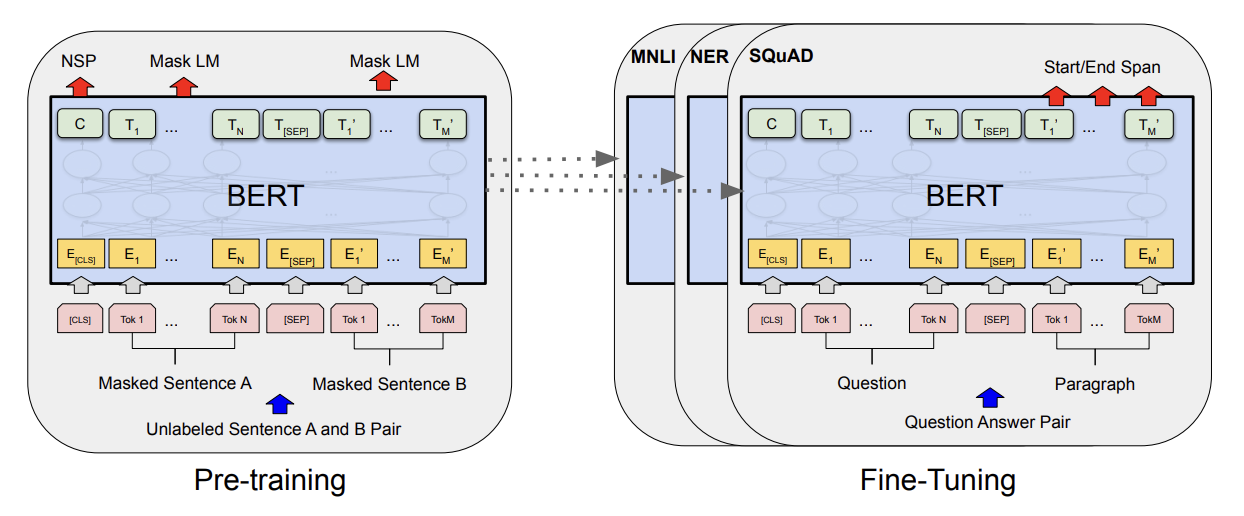
\includegraphics[width=0.8\textwidth]{chapter-2/bert.png}
    \caption{Arsitektur \textit{BERT} \parencite{bert}}
    \label{fig:bert}
\end{figure}

BERT merupakan \textit{pre-trained model} sehingga telah dilatih pada sejumlah besar teks. Data latih BERT diambil dari BooksCorpus dan Wikipedia bahasa Inggris. Ini memungkinan BERT untuk mempunyai pengetahuan mendasar dalam tugas NLP. Ketika digunakan untuk tugas-tugas NLP spesifik, seperti klasifikasi teks atau pemahaman pertanyaan, BERT dapat disesuaikan dengan data tugas spesifik untuk meningkatkan kinerjanya.

Model ini dikembangkan dengan dua konfigurasi, yaitu BASE dan LARGE. BERT dengan konfigurasi BASE memiliki 12 \textit{layer encoder} yang mempunyai 768 \textit{hidden layer} pada FFNN dan 12 \textit{attention heads}. Sedangkan, untuk konfigurasi BERT LARGE memiliki 24 \textit{layer encoder} yang mempunyai 1024 \textit{hidden layer} pada FFNN dan 16 \textit{attention heads}.

\subsection{IndoBERT}
\label{sec:indobet}

Meskipun terdapat lebih dari 200 juta pengguna bahasa Indonesia, bahasa tersebut kurang terwakili di NLP \parencite{indolem}. Sehingga, IndoBERT muncul untuk memperbaiki situasi ini. IndoBERT adalah adaptasi dari model BERT yang khusus dilatih untuk bahasa Indonesia. Mengingat keunikan dan kompleksitas bahasa Indonesia, memiliki model yang khusus dilatih untuk bahasa ini sangat penting untuk memastikan kinerja yang optimal pada tugas-tugas NLP yang berfokus pada bahasa Indonesia \parencite{indolem}.

\begin{figure}[ht]
    \centering
    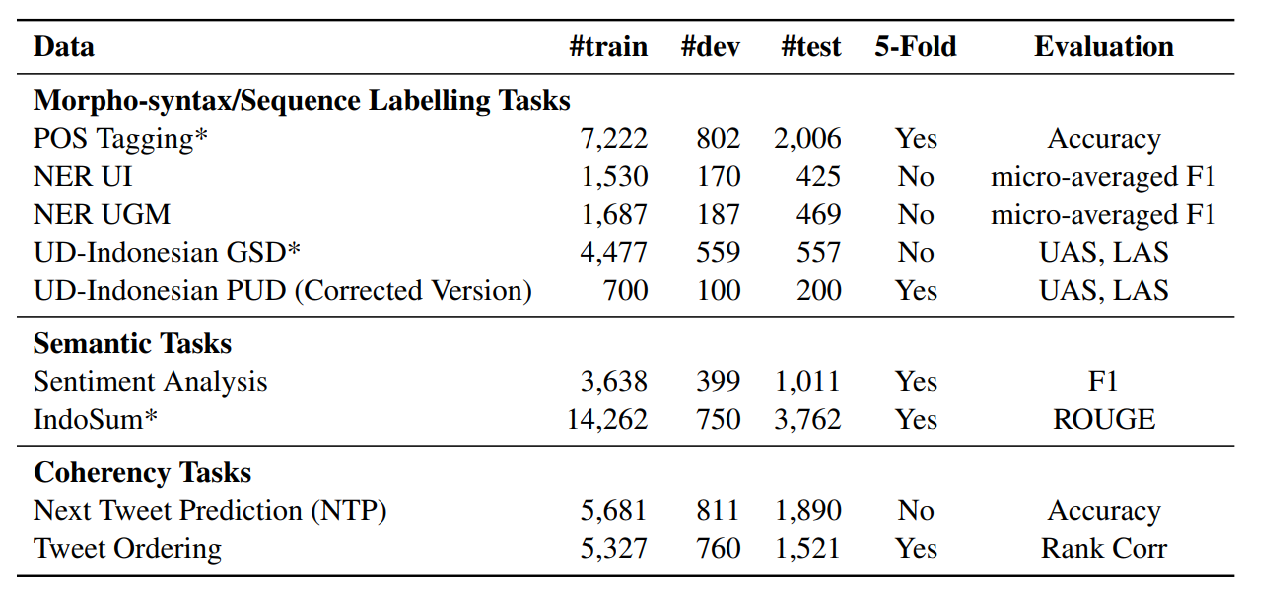
\includegraphics[width=0.8\textwidth]{chapter-2/indobert_dataset.png}
    \caption{\textit{Dataset} pada IndoBERT \parencite{indolem}}
    \label{fig:indobert_dataset}
\end{figure}

IndoBERT berbasis pada \textit{pre-trained model} BERT yang dilatih secara khusus pada \textit{dataset} berbahasa Indonesia, seperti yang bisa dilihat pada Gambar \ref{fig:indobert_dataset}. Tugas NLP yang dilatih pada IndoBERT dibagi menjadi tiga, yaitu \textit{sequence labelling}, \textit{semantic}, dan \textit{coherency}. Untuk \textit{sequence labelling} terdapat tiga tugas, yaitu \textit{part-of-speech} (POS) \textit{tagging}, \textit{named entity recognition} (NER), dan \textit{dependency parsing}. Lalu, untuk \textit{semantic} terdapat dua tugas, yaitu \textit{sentiment analysis} dan \textit{summarization}. Terakhir, untuk \textit{coherency} terdapat dua tugas, yaitu \textit{next tweet prediction} dan \textit{tweet ordering}.

\begin{figure}[ht]
    \centering
    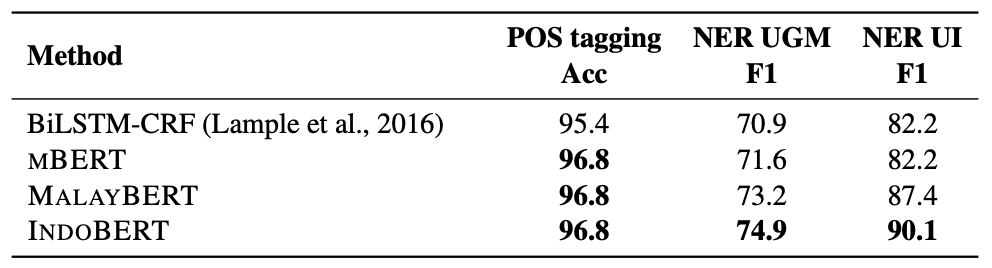
\includegraphics[width=0.8\textwidth]{chapter-2/indobert_pos.png}
    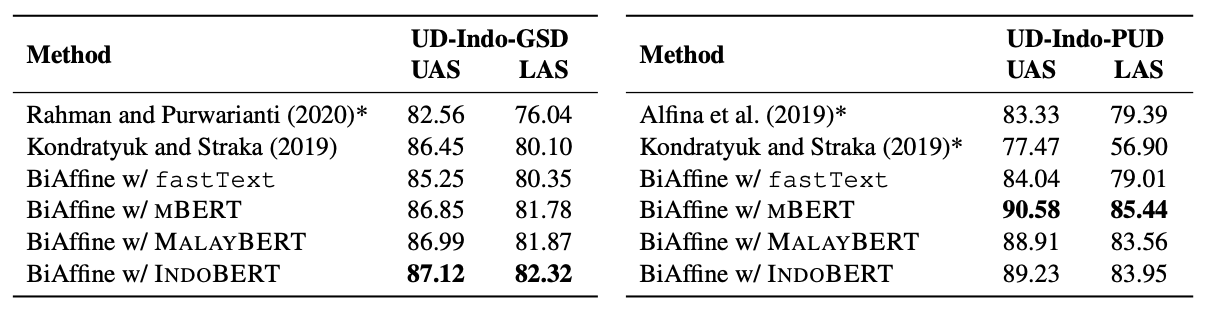
\includegraphics[width=0.8\textwidth]{chapter-2/indobert_dependency_parsing.png}
    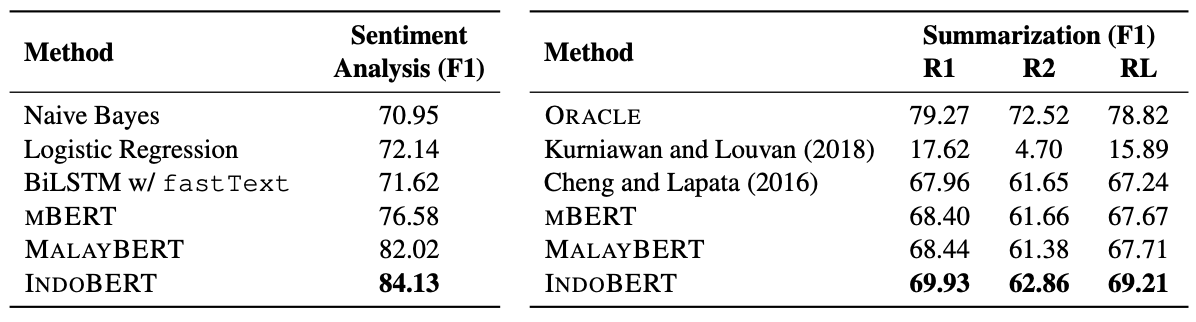
\includegraphics[width=0.8\textwidth]{chapter-2/indobert_semantic.png}
    \caption{Hasil Evaluasi IndoBERT \parencite{indolem}}
    \label{fig:indobert_evaluation}
\end{figure}

Untuk melakukan evaluasi terhadap model, dilakukan perbandingan dengan model lain. Pada penelitian ini, digunakan \textit{multilingual} BERT (mBERT) dan MalayBERT yang di-\textit{fine-tune} dengan bahasa Indonesia sebagai pembanding \parencite{indolem}. Hasilnya, IndoBERT kebanyakan unggul di setiap tugas. Selain dari tugas \textit{part-of-speech} (POS) \textit{tagging} dan \textit{next-tweet prediction} masih bisa dilakukan peningkatan \parencite{indolem}. Hasil evaluasi secara detail dapat dilihat pada Gambar \ref{fig:indobert_evaluation}.
